\newcommand{\Email}{\mbox{mariolink@hotmail.de}}
\newcommand{\Address}{\mbox{Kummerower Ring 71}, \mbox{12619 Berlin}}
\newcommand{\Mobile}{\mbox{+49 176 96 69 84 83}}
\newcommand{\Tel}{\mbox{+49 30 92 88 936}}
\newcommand{\Signature}{\mbox{}\\
\includegraphics[scale=0.5]{signature.png}\\Berlin, \today}

\title{Julia Grafik Engine}
\author{Mario Link}
\date{\today}

\documentclass[11pt]{article}

% Text- und Font-Encoding:
%\usepackage[T1]{fontenc}
%\usepackage{german}
\usepackage[EU1]{fontenc}
\usepackage[utf8]{inputenc}
%\usepackage{fontspec}
\usepackage[german]{babel}

%\usepackage{arial}
\renewcommand{\familydefault}{\sfdefault}

%\usepackage{tgtermes}
% Worttrennung
%\hyphenation{er-reich-en}

\pagestyle{empty}

%\usepackage{parskip}

% table
\usepackage{tabu}
\usepackage{tabularx}
%\usepackage{tocloft}

%\renewcommand\cftchapaftersnum{.}% adds dot after chapter title in ToC
%\renewcommand\cftchapdotsep{\cftdotsep}% adds leader dots from chapter titles to page numbers
%\renewcommand{\cftsecaftersnum}{.}% adds dot after section title in ToC

%lists
\usepackage{paralist}
%\usepackage{enumitem}
%\setlist{nosep} % or \setlist{noitemsep} to leave space around whole list

%\usepackage{bookman}
%\usepackage{newcent}
%\usepackage{mathpazo}
%\usepackage{mathptmx}
%\usepackage{chancery}
%\usepackage{helvet}
%\usepackage{charter}
\usepackage{xfrac}

% Grafiken einbinden
\usepackage{pgf}
\usepackage{tikz,ifthen,fp,calc}
\usepackage{graphicx}
\usepackage{pdfpages}
\usepackage{pgfplots}
\usepackage{pgfplotstable}

\usetikzlibrary{patterns}
\usetikzlibrary{backgrounds}

\usepackage[pages=some,scale=1,angle=0,opacity=1.0]{background}

% Layout ändern
% a4paper
% letterpaper
% legalpaper
% left, right, top, bottom
% textwidth, textheight
% footskip
% marginparsep, marginparwidth
%\usepackage[paperwidth=23cm,paperheight=42cm]{geometry}
\usepackage[a4paper,twoside, nohead,
  %paperwidth=23cm,paperheight=42cm,
  %textheight=24cm,footskip=2.5cm,
  inner=0cm,outer=0cm,
  top=2cm,bottom=2cm,left=2cm,right=2cm]{geometry}

% Zeilenabstand
\usepackage{setspace}
\setstretch{1.0}
\setlength\parindent{0pt}
\setlength{\parskip}{2pt}
\renewcommand{\baselinestretch}{1.5}

\usepackage[absolute,overlay]{textpos}
  \setlength{\TPHorizModule}{1mm}
  \setlength{\TPVertModule}{1mm}


\usepackage{listings} %code
\usepackage{color} % Farbe
\usepackage[unicode]{hyperref}
%\usepackage{bookmark}

\definecolor{green}{rgb}{0.0, 1.0, 0.0}
\definecolor{black}{rgb}{0.0, 0.0, 0.0}
\definecolor{page}{RGB}{100, 130, 150}
\definecolor{bg}{RGB}{70, 100, 120}
\definecolor{section}{RGB}{70, 100, 120}
\definecolor{content}{RGB}{230, 230, 255}
\definecolor{title}{RGB}{0, 51, 51}
\definecolor{MetallicGold}{RGB}{212, 175, 55}
\definecolor{book}{RGB}{200 200, 200}

\definecolor{dkgreen}{rgb}{0,0.6,0}
\definecolor{gray}{rgb}{0.5,0.5,0.5}
\definecolor{mauve}{rgb}{0.58,0,0.82}

\lstset{frame=tb,framerule=0pt,
  framextopmargin=3pt,
  framexleftmargin=10pt,
  framexbottommargin=3pt,
  language=R,
  aboveskip=3mm,
  belowskip=3mm,
  showstringspaces=false,
  columns=flexible,
  basicstyle={\small\ttfamily},
  numbers=none,
  numberstyle=\tiny\color{gray},
  keywordstyle=\color{blue},
  commentstyle=\color{dkgreen},
  stringstyle=\color{mauve},
  backgroundcolor=\color{content},
  breaklines=true,
  breakatwhitespace=true,
  tabsize=3
}

\hypersetup{
    bookmarks=true,         % show bookmarks bar?
    unicode=false,          % non-Latin characters in Acrobat’s bookmarks
    pdftoolbar=true,        % show Acrobat’s toolbar?
    pdfmenubar=true,        % show Acrobat’s menu?
    pdffitwindow=false,     % window fit to page when opened
    pdfstartview={FitH},    % fits the width of the page to the window
    pdftitle={Julia Grafik Engine},    % title
    pdfauthor={Mario Link},     % author
    pdfsubject={Julia Grafik Engine},   % subject of the document
    pdfcreator={Mario Link},   % creator of the document
    pdfproducer={Mario Link}, % producer of the document
    pdfkeywords={Julia, OpenGL, Python, Tests, Grafik Engine, Entwicklung}, % list of keywords
    pdfnewwindow=true,      % links in new PDF window
    colorlinks=true,       % false: boxed links; true: colored links
    linkcolor=section,          % color of internal links (change box color with linkbordercolor)
    citecolor=gray,        % color of links to bibliography
    filecolor=red,      % color of file links
    urlcolor=blue           % color of external links
}

% Übeschriften-Einstellungen
\usepackage{sectsty}
\allsectionsfont{\sffamily\color{section}}

% Bild- und Tabellenbeschriftungen
\usepackage[labelsep=newline,labelfont=bf,figurename=Abb.]{caption}

\usepackage{everypage}
\usepackage{xcolor}
\usepackage{lipsum}

\newlength\inset
\inset=1in\relax

\usepackage[compact]{titlesec}
\titlespacing{\section}
{0pt}{1.0ex plus 1.0ex minus 0.2ex}{0.75ex plus 0.2ex}
\titlespacing*{\subsection}
{0pt}{1.0ex plus 1.0ex minus 0.2ex}{0.75ex plus 0.2ex}
\titlespacing*{\subsubsection}
{0pt}{1.0ex plus 1.0ex minus 0.2ex}{0.75ex plus 0.2ex}

%%%

% commands
\newcommand{\xhline}[1]{\noindent\makebox[\linewidth]{\rule{\textwidth}{#1}}}

\newcommand{\listdot}{\fontsize{7pt}{0}\selectfont>}
\newcommand{\smallbold}[1] {{\fontseries{sbc}\selectfont #1}}

\newcommand{\source}[1]{\caption*{Quelle: {#1}} }

\begin{document}
\pagecolor{page}

\vspace*{-5.0cm}
\hspace{0pt}
\vfill
\begin{center}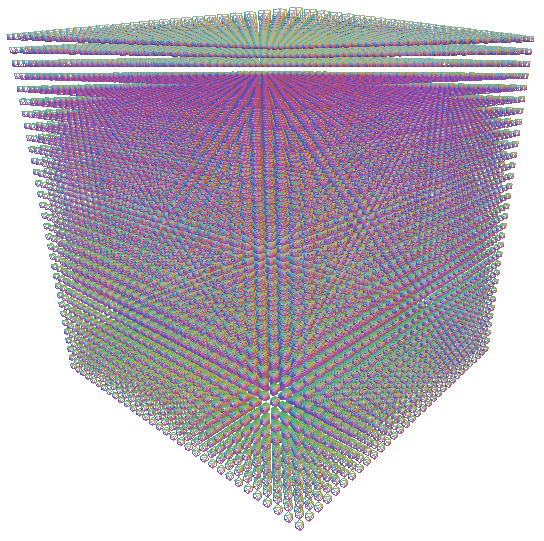
\includegraphics[scale=1.0]{title.png}\end{center}
\vspace*{1.0cm}
{
\fontsize{30}{60}\selectfont\color{white}
\textbf{Julia Grafik Engine}\\
\vspace*{0.5cm}\\
\fontsize{25}{60}\selectfont
Independent Coursework 2\\
\vspace*{0.5cm}\\
\fontsize{20}{60}\selectfont
Mario Link (s0536176)
}
\vfill

\afterpage{\nopagecolor}
\newpage

\tableofcontents

\newpage

\maketitle

\section{Einleitung}
Das Dokument beschreibt die Idee der Entwicklung einer Grafik Engine in der Sprache Julia. Das Ziel ist es zu zeigen ob Julia für Entwicklung von Grafik Engines geeignet ist. Ein weiteres Ziel ist einen Vergleich zu anderen Sprachen aufzustellen und welche Vor- und Nachteile sich mit dieser Sprache ergibt.

\subsection*{Problemstellung/Fragestellung}
Ist die Entwicklung einer Grafik Engine in Julia einfacher als in anderen Sprachen wie z.B. Python?

\subsection*{Weitere Fragen}
\begin{flushleft}
\begin{compactitem}
\item Welche Vor-/Nachteile ergeben sich bei der Verwendung von Julia statt anderen Sprachen wie z.B. Python? Gibt es Performance unterschiede? 
\item Was sind der Vor-/Nachteile von JIT?
\item Sind Design Pattern in Julia umsetzbar?
\item Wie sieht Parallelisierung, Garbage Collection und Unit Tests in Julia aus?
\item Wie gut sind Julia Projekte Skalierbar? (Blick in Zukunft: Weiterentwicklung zur Game Engine)
\end{compactitem}
\end{flushleft}

\subsection*{Ziel}
Demonstrationssystem (Grafik Engine) in Julia entwickeln, Arbeitsaufwand und Performance bewerten.

\newpage

\section{Basics}
\subsection{Was ist Julia?}
Julia ist eine Hoch-Level, hoch-performante dynamische Sprache für numerisches Rechnen. Es stellt einen hochentwickelten Compiler, verteilte parallelisierte Ausführung, numersiche Genauigkeit und eine umpfangreiche mathematische Funktionsbinliothek zur Verfügung. Julia's Basis-Bibliothek wurde größtenteils selbst in Julia geschrieben. Julia integriert zudem optimierten (bestmöglichen) Code von Open Source C und Fortran Bibliotheken für lineare Algebra, Generierung von Zufallsnummern, Singal und String Verarbeitung. Zusätzlich bietet die Julia Entwickler Community eine Reihe von externen Packeten (Modulen) durch den eingebauten Julia Packetmanager an. IJulia ist eine Kollaboration zwischen Jupyter und Julia Communities und stellt ein mächtiges Browser-basiertes grafisches Notebook mit Schnittstelle zu Julia zur Verfügung. Julia's Stärken zeigen sich vorallem durch den auf LLVM-basierten hoch-performanten just-in-time (JIT) Compiler, der kombiniert mit dem Julia Sprach-Design eine C nahe Performance ermöglicht. Julia Programme sind durch den multiplen Dispatch organisiert, der  den Einsatz für verschiedene Kombinationen von Argumenttypen für überladete Funktionen unterstützt. Die Sprache kann als dynamische Bibliothek (shared library) gebaut werden. Einfache Aufrufe zu externen Funktionen in C und Fortran aus dynamischen Bibliotheken sind ebendso möglich, ohne das Wrapper Code geschrieben oder existierener Code recompiliert werden muss. Julia ist Open Source (Core Bibliothek enthält MIT Lizenz). Weitere Lizenzen wie GPL, LGPL, and BSD werden von anderen Bibliotheken genutzt.\\ (siehe \url{https://julialang.org/#free-open-source-and-library-friendly})\\

\hypertarget{basics}{Zusammenfassung der Features:}\\
\noindent\minipage[t]{\dimexpr0.5\linewidth\relax}

\begin{flushleft}
\begin{compactitem}
\item Multiples Dispatch
\item Dynamisches Typ-System
\item Gute performance (nahe C)
\item Built-in package manager
\item Lisp-like Macros und andere Vorteile der Metaprogrammierung
\item Call Python Funktionen (PyCall)
\item Call C Funktionen (direkt, keine Wrapper)
\item Mächtige shell-ähnliche Fähigkeiten für das Managen von Prozessen
\end{compactitem}
\end{flushleft}

\endminipage\hfill
\noindent\minipage[t]{\dimexpr0.5\linewidth\relax}

\begin{flushleft}
\begin{compactitem}
\item Designed für Paralellität und Cloud Computing
\item Coroutinen: leichtgewichtetes ''grünes'' Threading
\item Benutzerdefinierte Typen (schnell und kompakt wie eingebaute Basis Typen)
\item Automatische und effiziente Code Generierung
\item Elegante und erweierbare Konvertierung und Promotionen für numerische und andere Types
\item Effizienter Support für Unicode (UTF-8)
\item MIT Lizenz: frei und Open Source
\end{compactitem}
\end{flushleft}

\endminipage\hfill\\
\newpage

\subsection{Was ist LLVM?}
LLVM (Low Level Virtual Machine)ist eine modulare Compiler-Unterbau-Architektur mit einem virtuellen Befehlssatz, einer virtuellen Maschine, die einen Hauptprozessor virtualisiert. Es besteht aus einer Sammlung von Compiler und Toolchain Technologien für die Entwicklung von Compiler Back- und Frontends. LLVM ist in C++ geschrieben und wird zur Optimierung von Compilerzeit, Linkzeit, Laufzeit und Leerlaufzeit herangezogen.\\

\begin{figure}[h]
\begin{center}
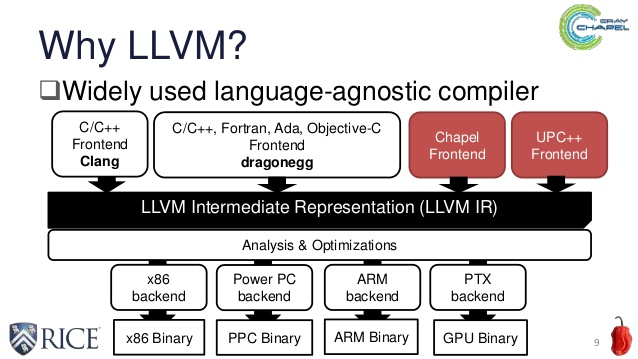
\includegraphics[scale=0.5]{llvm.jpg}
\source{\href{https://image.slidesharecdn.com/ahayashi20151115-151115205825-lva1-app6891/95/llvmbased-communication-optimizations-for-pgas-programs-9-638.jpg?cb=1519689486}{llvmbased-communication-optimizations-for-pgas-programs}}
\end{center}
\end{figure}

\newpage
\begin{figure}[h]
\begin{center}
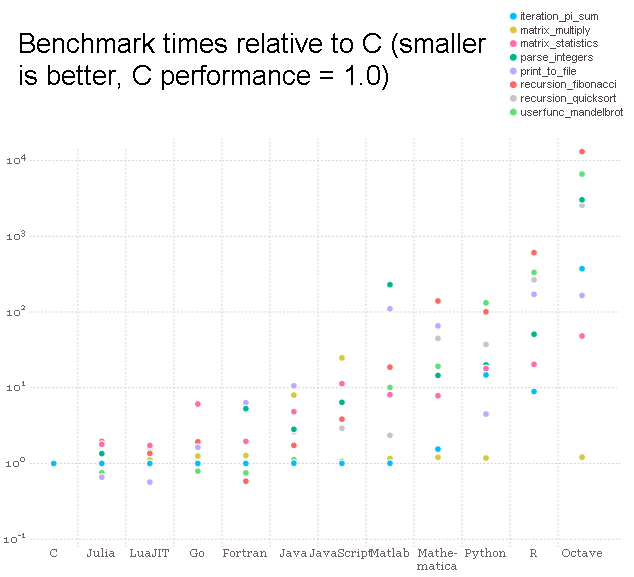
\includegraphics[width=\textwidth]{benchmark.png}
\caption{Vergleich von Micro-benchmarks zwischen verschiedenen Sprachen: C, Fortran, Julia, Python, Matlab/Octave, R, JavaScript, Java, Lua, Mathematica.}\label{imageLabel}
\source{Micro-benchmarks \url{https://julialang.org/}}
\end{center}
\end{figure}

\newpage
\subsection{Dokumentation}
Julias Dokumentation ist auf Seite \url{https://docs.julialang.org/en/stable/} einsehbar.\\
Ein kleine Hilfe für den schnellen Einstieg bietet die Seite \url{https://learnxinyminutes.com/docs/julia/}

\subsection{Beispiel Code}
\noindent\begin{minipage}{\textwidth}
Die ausführbare Julia Datei (julia.exe) liefert eine interaktive Befehlsoberfläche (Konsole) genannt REPL (read-eval-print loop). In dieser Konsole kann Julia Code direkt ausgeführt werden. Desweiteren können Julia Skripte angelegt und per julia.exe ausgeführt werden. Die Vorgehensweise:

1. Ein Batch Script run.bat schreiben und den Pfad zur julia.exe und dem Script angeben.
\begin{lstlisting}
@echo off
"C:/Users/\%username\%/AppData/Local/Julia-0.6.0/bin/julia.exe" "main.jl"
pause
\end{lstlisting}
\end{minipage}

\noindent\begin{minipage}{\textwidth}
2. Das Script main.jl anlegen.
\begin{lstlisting}
println("Hello World!")
\end{lstlisting}
\end{minipage}

3. Die run.bat starten und das Ergebnis bewundern.

\subsection{Julia Box - Julia Code im Web}
Julia kann auch im Web ausgeführt werden, siehe \url{https://www.juliabox.com/}.

\subsection{Design Pattern}
\noindent\begin{minipage}{\textwidth}
Anders als in Java existiert in Julia die Behandlung von Klassen, private und public Definitionen nicht. In Julia existieren Module, Structs, Types und Funktionen. Module könnten als public static Class betrachtet werden. Der Unterschied von Struct zu Type ist, dass Struct Objekte unveränderlich sind.

\begin{lstlisting}
julia> module MyApp end
julia> type MyObject end
julia> struct MyImmutableObject end
\end{lstlisting}
\end{minipage}

\noindent\begin{minipage}{\textwidth}
Die Zugehörigkeit von Funktionen zu Structs/Types lässt sich nur funktional über den Funktionsparameter lösen.
\begin{lstlisting}
julia> function myFunction(this::MyObject, value::Int) end
\end{lstlisting}
\end{minipage}

\noindent\begin{minipage}{\textwidth}
Allerdings kann die Zugehörigkeit durch einen Workround, durch das Speichern von anonymen Funktionen, geregelt werden:
\begin{lstlisting}
julia> type MyObject
	x::Int
	getX::Function # public method
	function MyObject()
		this = new()
		this.x = 0
		this.getX = ()->this.x
		this # return object
	end
end
julia> MyObject().getX()
\end{lstlisting}
\end{minipage}

\noindent\begin{minipage}{\textwidth}
Private Methoden können mit diesem Ansatz gelöst werden:
\begin{lstlisting}
julia> let
	global brotherB
	function brotherA(x="I am private!")
		println("brotherA: ",x)
	end

	function brotherB()
		println("brotherB: I am public!")
		brotherA("Bro... i was hiding!!!")
	end
end
julia> brotherA()
ERROR: UndefVarError: brotherA not defined
julia> brotherB()
brotherB: I am public!
brotherA: Bro... i was hiding!!!
\end{lstlisting}
\end{minipage}

Informationen zum Scope können hier gefunden werden: \url{https://docs.julialang.org/en/stable/manual/variables-and-scoping/}

\subsection{Garbage Collection}
Der Garbage Collector erfolgt nach einer gewissen Zeit automatsich. Allerdings kann mit dem Befehl gc() der Garbage Collector sofort ausgeführt werden.

\subsection{Unit Tests}
\noindent\begin{minipage}{\textwidth}
Tests können in Julia können z.B. mithilfe des Macro Befehls @test aus dem Modul Base.Test ausgeführt werden (\url{https://docs.julialang.org/en/stable/stdlib/test}).
\begin{lstlisting}
julia> using Base.Test
julia> @test 1 == 1
Test Passed
julia> @test 1 == 2
Test Failed
  Expression: 1 == 2
   Evaluated: 1 == 2
ERROR: There was an error during testing
\end{lstlisting}
\end{minipage}

\subsection{Parallelisierung}

\noindent\begin{minipage}{\textwidth}
Mit Ausführung von ''julia.exe -p 10 myScript.jl'' kann ein Script über mehrere Prozesse (z.B. 10) gestartet werden:
\begin{lstlisting}
@everywhere function write(i)
  Libc.systemsleep(5)
  (myid(),i)
end
list = Future[]
println("Write")
for i=1:nprocs() println("$i"); push!(list, @spawn write(i)) end
println("Read - Wait ~ 5 sec")
for entry in list println(fetch(entry)) end
\end{lstlisting}
\end{minipage}

\noindent\begin{minipage}{\textwidth}
Threads lassen sich bisher nur experimentell mit
Umgebungsvariable JULIA\_NUM\_THREADS=4 (4 Threads) ausführen:
\begin{lstlisting}
a = zeros(10)
Threads.@threads for i = 1:10
	a[i] = Threads.threadid()
end
\end{lstlisting}
\end{minipage}

\subsection{JIT und Power of Eval}
\noindent\begin{minipage}{\textwidth}
Der JIT Compiler ermöglich die Ausführung der des Codes zur Laufzeit. Demnach werden Beispielsweise include() Anweisungen in Funktionen merhfach ausgeführt.

\begin{lstlisting}
julia> function inlucdeAll()
	include("myCode1.jl")
	include("myCode2.jl")
	include("myCode3.jl")
end
julia> for i:10 #include all code 10 times
	inlucdeAll()
end
\end{lstlisting}
\end{minipage}

\noindent\begin{minipage}{\textwidth}
Allerdings kann es hierbei zu Problemen kommen, wenn in dem includierten Code Struct oder Typen definiert sind. Eine Redefinition dieser Objekte ist nicht möglich, da diese an das momentane Modul festgebunden  sind. Erst ein komplettes überschreiben des Moduls ermöglicht eine Redefinition.
\begin{lstlisting}
julia> type MyObject end
julia> type MyObject x::Int end
ERROR: invalid redefinition of constant MyObject
\end{lstlisting}
\end{minipage}

\noindent\begin{minipage}{\textwidth}
Mit der Anweisung eval() lässt sich dynamischen Julia Code generieren. Die Funktion eval benötigt einen Symbol Parameter, um neuen Code zu generieren. Durch die Funktion parse() lässt sich ein Befehl als String Objekt in einen Symbol Objekt umwandeln.
\begin{lstlisting}
julia> function myFunction() end
julia> myFunction() #keine Ausgabe
julia> eval(parse("function myFunction(); println(\"Hi!\"); end"))
julia> myFunction() #Ausgabe "Hi!"
\end{lstlisting}
\end{minipage}

\subsubsection{Was sind die Vor- und Nachteile von JIT?}
Vorteil von JIT ist, dass der Code nicht noch einmal interpretiert werden muss, sondern direkt in Binärcode kompiliert wird. Dadurch wird sofort ein Ergebnis geliefert. JIT hat längere Ausführungszeit als AOT (Ahead of Time) Systeme. Liefert jedoch deutlich besseren Code. Durch die extistieren Systemprofile werden die bestmöglichen Instruktionen für das Zielsystem bei der Kompilerung ausgewählt. AOT liefert eine schnellere Ausführungsgeschwindigkeit als JIT, verbraucht jedoch mehr Arbeits- und Festplattenspeicher und muss alle Möglichen Systemprofile durchgehen (Quelle: \url{https://www.thoughtco.com/definition-of-compiler-958198}).

\section{Julia vs Python}

\subsection{Artikel 'Giving up on Julia'}

In meiner Recherche bin ich auf den Artikel \textbf{Giving up on Julia} (\url{http://www.zverovich.net/2016/05/13/giving-up-on-julia.html}) gestoßen. Der Artikel ist 2 Jahre alt und bezieht sich auf Julia 0.4. Er beschreibt Probleme von Julia und zeigt nur wenig Testszenarien als Beweis. Der Author bemängelte die Microbenchmarks auf der Julia Webseite, sowie:

\begin{flushleft}
\begin{compactitem}
\item Performance Probleme bei StartUp Zeit und JIT lags
\item Undurchsichtige Syntax und Probleme mit der Zusammenarbeit mit anderen Sprachen
\item Schwache Textformatierungshilfen in der Sprache sowie fehlen von guten Unit Test Frameworks
\item standardmäßig unsicheres Interface zu nativen Schnittstellen (APIs)
\item Unnötig komplizierte Code-Basis und unzureichende Aufmerksamkeit beim BugFixing
\end{compactitem}
\end{flushleft}

Ein Test zeigt ein ''Hello World'' Program und ein weiterer Test einen Schnittstellenaufruf mit ccall(). In den Testszenarien wurde keine direkten Gegenüberstellung von Python und Julia gezeigt. 

Desweiteren schlägt er vor Python Funktionen zu optimieren (siehe \url{https://www.ibm.com/developerworks/community/blogs/jfp/entry/Python_Meets_Julia_Micro_Performance})

\subsection{Artikel 'Updated Analysis'}

Als Gegendarstellung enstand der Artikel \textbf{Updated Analysis} (\url{https://tk3369.wordpress.com/2018/02/04/an-updated-analysis-for-the-giving-up-on-julia-blog-post/}), der durch direkte Gegenüberstellung zeigt, dass Python gegenüber Julia schlechter abschneidet. Der Author dieses Artikels kritisiert den Author des \textbf{Giving up on Julia} Artikels. Dieser habe die Darstellung nur verwendet, um auf seinen Block ''How To Make Python Run As Fast As Julia'' aufmerksam zu machen und nicht das eigentliche Problem der Gegenüberstellung behandelt. 
Die Gegendarstellung in diesem Artikel zeigt Tests mit der Berechnung von Fibonacci-Zahlen, Quicksort, Mandelbrot Set und Integer Parsing. Desweiteren bezieht er sich auf die Argumente im \textbf{Giving up on Julia} Artikel wie Syntax, Sicherheit, Textformatierung beim Printf, Unit Tests und weiteren.
In allen Tests schneidet Julia besser ab als Python oder CPython.

\subsection{Artikel 'Observations'}

Bei diesem Artikel (\url{https://medium.com/@Jernfrost/python-vs-julia-observations-e61ee667fa95}) bezieht sich dieser Author auf die allgemeine Handhabung von Julia und Python. Er vergleicht REPL, die Interaction mit Arrays, die Integration von Shell Befehlen und anderen Eigenschaften der Syntax. Julia schneidet hier nach seiner Meinung sehr gut ab. Der Author erkennt an, dass Python eine deutlich größere Community besitzt als Julia und dadurch einen Vorteil erhält. Er ist jedoch überzeugt, dass Julia einene besseren Einstieg ermöglicht als Python. 

\subsection{Zusammenfassung}

Julia ist eine sehr neue Sprache und enthält viele Vorteile aus anderen Sprachen und weniger deren Nachteile. Julia ist aus dem Kenntnisstand erfahrender Entwickler aus aller Welt enstanden, die früher in Matlab, C++, Java, R, Python und anderen Sprachen programmiert haben. Ich sehe darin ein deutlichen Vorteil, da unterschiedlich Erfahrungswerte hier zusammenkommen.\\

\noindent\begin{minipage}{\textwidth}
Im Überblick - die Persöhnliche Einschätzung (Erfahrungswerte): (E = Einfachheit, Syntax, Style; U = Umpfang, Anzahl Bibliotheken; P = Performance zu C; A = investierter Aufwand/Zeit für einen Anwendungsfall)\\

\pgfplotstableread[col sep=comma]{
X,Y
Julia E,4
Python E,3
Julia U,2
Python U,4
Julia P,3
Python P,1
C-Python P,3
Julia A,4
Python A,3
Dummy,0
}\skills
{
\begin{tikzpicture}[scale=1]
\begin{axis}[
	xmajorgrids,
    width=0.25\linewidth,
    height=150,%.5\textwidth,
    enlargelimits=false, %0.01,
    xbar interval=0.5,
    tick style={transparent},
    y dir=reverse,
    xtick=data,
    yticklabels from table={\skills}{X},
    xticklabels={1,2,3,4},
    xlabel={Bewertung als grobe Note},
    axis y line*=left,
    major y grid style={
            transparent,
    },
    %axis x line*=top,
   	%xticklabel pos=upper,
   	%xlabel shift = -1.5in,
    xmin=0,
    ymin=0,
    ]
\foreach \i in {Y}
{\addplot[top color=page, bottom color=white] table [y expr=\coordindex, x=\i] {\skills}; }
\end{axis}
\end{tikzpicture}
}
\end{minipage}

\section{Entwicklung}
Für die Entwicklung wurden zwei Programme geschrieben. Das erste repräsentiert die Herangehensweise der Entwicklung einer Grafikengine und das zweite die Herangehensweise eines optimierten Renderalgorithmus für einen speziellen Fall (Das Rendern von vielen Blöcken/Cubes).

\subsection{Projekte einrichten}

\textbf{Herunterladen:}\\
1. Julia 0.6: \url{https://julialang.org/downloads/}\\
2. Julia OpenGL: \url{https://github.com/Gilga/JuliaOpenGL}\\
3. Julia Grafik Engine: \url{https://github.com/Gilga/JGE}\\

\textbf{Installieren:}\\
1. Julia 0.6 Setup ausführen\\
2. Bei den Projekten die dort enthaltene README.md lesen und Packete nachinstallieren mit:
\begin{lstlisting}
Julia> Pkg.add("Modulname hier einfügen")
\end{lstlisting}

Die Projekte wurden nur auf diesem System entwickelt und getestet:

\begin{flushleft}
\begin{compactitem}
\item Operating System: Windows 10 Home 64-bit
\item Processor: Intel(R) Core(TM) i7-4510U CPU @ 2.00GHz (4 CPUs), ~2.0GHz
\item Memory: 8192MB RAM
\item Graphics Card 1: Intel(R) HD Graphics Family
\item Graphics Card 2: NVIDIA GeForce 840M
\end{compactitem}
\end{flushleft}

Es wurde bevorzugt mit der NVIDIA Grafikkarte getestet (für bessere FPS Werte).

\subsection{Julia GrafikEngine}
Das Projekt ist so aufgeteilt das App bezogene Skripte und Objekte (wie Shader, Texturen, Szenenscript) im Root Verzeichnis des Projektes liegen und die Core Skripte für die Engine im source Ordner. Im source Ordner werden die Julia Versionen unterschieden (0.5, 0.6, usw.). In dem Ordner sollten der Source Code (im src Ordner), sowie Tests (im test Ordner) stehen. In meinem Fall habe ich aus Prioriäts- und Zeitgründen keine konkreten Skripttests geschrieben. Stattdessen wurden die Tests manuell über die Julia Konsole ausgeführt, um Probleme zu beheben. Allerdings existieren allgemeine Test Skripts im zweiten Projekt (JuliaOpenGL Projekt).\\
\noindent\minipage[t]{\textwidth}
Skripte und Ordner:\\
\noindent\minipage[t]{\dimexpr0.5\linewidth\relax}

\begin{flushleft}
\begin{compactitem}
\item scripts/input.jl - enthält Szenenbeschreibung
\item source/0.6/App.jl - Beschreibt den Aufruf des Programms und initialisiert den Prozess
\item source/0.6/CoreExtended.jl - enthält eine Sammlung von erweitere Kernfunktionen für viele Zwecke 
\item source/0.6/Environment.jl - legt Umgebung fest wie z.B. globale Pfade und Variablen. Ist derzeit leer und nicht von Bedeutung.
\item source/0.6/FileManager.jl - Behandelt Lese und Schreib Funktionen für Dateien, sowie ein Event wenn festgelegte Dateien verändert wurden.
\item source/0.6/MatrixMath.jl - enthält mathematische Operationen für Matritzen und Vectoren
\item source/0.6/LoggerManager.jl - enthält die Vewaltung des Loggings
\item source/0.6/JLScriptManager.jl - Verwaltet das Sktiptsystem
\end{compactitem}
\end{flushleft}

\endminipage\hfill
\noindent\minipage[t]{\dimexpr0.5\linewidth\relax}

\begin{flushleft}
\begin{compactitem}
\item source/0.6/RessourceManager.jl - Verwaltet Ressourcenpfade
\item source/0.6/ThreadFunctions.jl - enthält erweiterte Thread Funktionen
\item source/0.6/ThreadManager.jl - Verwaltet Threads
\item source/0.6/TimeManager.jl - enthält Zeit Funktionen
\item source/0.6/WindowManager.jl - Verwaltet das Programmfenster (GLFW)
\item source/0.6/JLGEngine.jl - Verwaltet die Zuordnung der Skripts für die Engine
\item source/0.6/JLGEngine/LibGL/ - enthält Skripte zu OpenGL, repräsentiert Schnittstelle OpenGL
\item source/0.6/JLGEngine/ModelManager - einfache Gruppierung zur Übersicht enthält Skripte für Meshfunktionen wie z.B. das Laden von OBJ Dateien
\end{compactitem}
\end{flushleft}

\endminipage\hfill\\
\endminipage\hfill\\
\newpage
Mit der GrafikEngine wird eine 3D Szene gebaut die verschiedene Objekte anzeigen kann. Zum Beispiel kann ein Würfel mit einem Mandelbrot Shader angezeigt werden. Ein anderer Würfel trägt eine Textur und ein weiterer Würfel tarnt sich als Kugel (durch einen Shadertrick).
Transparente Objekte sind ebenfalls möglich. In der Szene kann der Betrachter die Kamera bewegen und sich umschauen. Die 3D Szene wird im Script \textbf{scripts/input.jl} beschrieben. Dort wird die Zuordnung von Objekten und Eigenschaften festgehalten. Bei einem Bearbeiten und Speichern der Datei wird das Programm automatsich die Szene neu Laden und die Veränderungen der Szene übernehmen. Die GrafikEngine ist so aufgebaut, dass für jedes logische Grafikobjekt wie z.B. Shader, Kamera, Mesh, Texture, usw. Manager Module existieren. Dadurch wird die Verwaltung einfacher und es können später optimierte Methoden hinzugefügt werden. Diese Skripte sind im \textbf{source/0.6/JLGEngine} Ordner zu finden. Die Renderszene wird durch ein Render Objekt (Renderer) verwaltet. Dieser enthält als Komponenten Eigenschaften (Meshdaten, Transformation, Texturen, usw.) für das jeweilige Objekt, dass gerendert werden soll. Das input.jl Script wird durch das eingebaute Skriptsystem verwaltet. Hierbei wird bei der Aktualisierung der input.jl Datei das zum Script repräsentierende Julia Modul überschrieben. Vor dem Aufruf des Renderprocesses werden Event Methoden (wie z.B. OnStart, OnUpdate) vordefiniert und Events werden an das Modul übergeben, sodass im Script die Behandlung von Events möglich ist. Events vom Programmfenster (GLFW) (z.B. OnKey) werden an das Script mitübergeben.

\subsection{JuliaOpenGL}
In diesem Projekt sind alle benötigten Skripte im Root Verzeichnis. Die Renderszene ist in der main.jl enthalten. In der Entwicklung wurde erkannt, dass der ursprungliche Ansatz des Grafikengine Konzepts für spezielle Fälle (wie Optimierung) ungeeignet ist. Eine sehr gute Grafikengine kann demnach nur über mehrere Entwicklungsphasen entstehen und wenn solche Spezialfälle mitberücksichtigt werden. In meinem Fall war es das Rendern von 128³ Blöcken (Cubes). Mit der OpenGL Draw Methode glDrawArrays() lassen sich nur Werte von 1-6 FPS maximal auf meinem System erreichen. Demnach wurde hier ein Optmierungsverfahren geschrieben. Es wird die Methode glDrawElementsInstanced() verwendet, ein Vertex, Fragment und Geometry Shader, sowie zwei Algorithmen (\textbf{Frustum Culling} und \textbf{Outside Only}). Die zwei Algorithem reduzieren die Anzahl der Blöcke bzw. Vertices. Dadurch entstehen großzügige Werte über 100 FPS bei 128³ Blöcken. Im Prinzip werden nur die sichtbaren Blöcke gerendert und nicht alle 128³. Bei glDrawElementsInstanced werden Instanzen einer Vertex Gruppe (z.B. Cube) mehrfach gerendert. Die Transformationsdaten werden über einen Buffer mitgegeben. Durch diese Methode wird ein mehrfach Aufruf einer OpenGL Funktion in einer Schleife (wie z.B. glDrawArrays) vermieden und das verursacht eine Performancesteigerung beim Rendern.
Das \textbf{Frustum Culling} Verfahren schneidet nur den sichtbaren Teil der Szene aus. Es repräsentiert die Kameraansicht (Viewport) und enthält sechs Ebenen (Oben, Unten, Rechts, Links, Vorne und Hinten). Nur innerhalb dieser Ansicht werden Objekte gerendert.
Bei dem \textbf{Outside Only} Verfahren werden versteckte Blöcke, die von anderen Blöcken umgeben sind, nicht gerendert. Der Geometry Shader ist standardmäßig beim mehrfachen Rendern schlechter als wenn Objekte mit festgelegten Strukturen (Vertices) gerendert werden. Allerdings ist er durch die Kombination von \textbf{Frustum Culling} und \textbf{Outside Only} Verfahren sehr stark, da nur noch Punktdaten an OpenGL übergeben werden müssen und erst bei Bedarf der Block bzw. eine Seite des Blocks erstellt wird. Dadurch lassen sich noch weniger Strukturen (Vertices) rendern.

\begin{center}
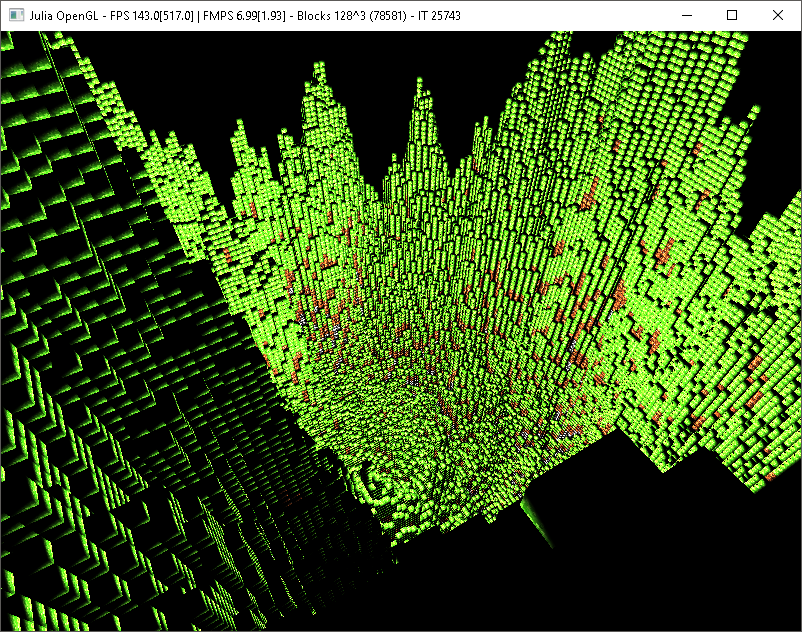
\includegraphics[width=0.9\textwidth]{status2.png}
\end{center}

\subsection{Warum wurde nicht GLAbstraction.jl verwendet?}

Die Bibliothek GLAbstraction.jl (\url{https://github.com/JuliaGL/GLAbstraction.jl}) war für meinen Ansatz eher ungeeignet, da sich die Bibliothek als Framework präsentiert und ich dadurch weniger nachvollziehen kann was eigentlich passiert. Da ich bereits eine GrafikEngine in C++ geschrieben und Kenntnisse mit nativen OpenGL Funktionen habe, wäre die Verwendung von GLAbstraction.jl für mich mit noch mehr Arbeit verbunden. Desweiteren bedient sich die Bibliothek momentan noch auf einer veralteten Bibliothek FixedSizeArrays.jl und dem Reactive.jl, was bei meinen Tests noch unzuverlässige Ergebnisse lieferte.

\subsection{Optimierung}
Es gibt die Möglichkeit mit Julia den GCC compiler auszuführen, um C-Code zu kompilieren. Der JuliaOptimizer im JuliaOpenGL Projekt wurde mit Visual Studio angelegt. Hier kann auch der Visual Stduio C++ Compiler verwendet werden, um optimierten Code zu schreiben. In Julia können über DLL-Schnittstellen C-Funktionen direkt angesprochen werden.

\subsection{Ausf\"uhrbare Dateien}
Mithilfe meines Build Skriptes lassen sich ausführbare Dateien erstellen: \url{https://github.com/Gilga/BuildExecutable.jl}\\
Das BuildScript sollte im gleichen Verzeichnis sein wo sich die zwei Projekte befinden. Per Batchdatei (build-(version).bat) lassen sich ausführbare Dateien generieren. In der Batch-Datei sollte der Pfad zu Julia richtig sein. Nach der Ausführung sollte ein build/(Julia-Version)/(Projectname)/ Ordner existieren und dort befindet sich die kompielierte ausführbare Datei.

\section{Probleme}
Ein großer Nachteil ist, dass es standardmäßig keine klare Möglichkeit gibt Julia Skripte in ausführbaren Dateien (executables) umzuwandeln. Demnach hab ich eine Fremdbibliothek (BuildScript) verwendet und diese für meine Verhältnisse angepasst (Github forked). Design Schwierigkeiten hatte ich am Anfang, da es keine Klassen und Vererbung gibt. Verebung lässt sich über komponentenbasiertes Design lösen. Fehlermeldung können schwer nachvollziehbar werden, wenn eval verwendet wird, aber das ist auch in anderen Sprachen ein bekanntes Problem. Wenn viel Code geschrieben wird, kann es passieren, dass unnützer Code entsteht und nicht aufgerufen wird. Das ist in Julia ein noch größeren Problem als in anderen Sprachen, da evtl. dieser Code sogar typ-falsch oder nicht extistent sein kann. Erst bei einem Aufruf kann Julia Probleme feststellen, daher sind automatiesierte Tests und Dokumentation sehr wichtig.\\
Ein ganz anderes Problem ist in meinem GrafikEngine Projekt das Skriptsystem. Derzeit ist es möglich im Script auf all Julia Funktionen zurückzugreifen. Das hat den Nachteil, dass das ganze Programm zweckentfremdet und somit als Schadsoftware umgeschrieben werden kann. Als mögliche Lösung könnten die zu verwenden Julia Funktionen eingeschränkt werden.

\section{Zusammenfassung}
Anhand dieses Projektes konnte ich zeigen, dass trotz der Größe sich das Projekt in zwei Projekte aufspalten und entwickeln lies. Ich habe keine jahrelangen Erfahrungswerte mit Julia, dennoch lernte ich die Sprache sehr schnell kennen. Ich würde Julia als ernsthaften Konkurrenten gegenüber Python ansehen, allerdings Bedarf es an etwas noch mehr Entwicklungzeit und Wachstum der Community, damit mehr Bibliotheken entsehen und weniger neu geschrieben werden muss, wie es auch in meinem Fall war. Die Möglichkeit Julia Skripte in ausführbaren Dateien (executables) umzuwandeln, sollte ein Bestandteil des Core Systems sein. Bisher ist es nur über externe Libraries (wie z.B. meiner eigenen) möglich. Desweiteren gibt es in vielen Modulen noch Optimierungsbedarf, um die Ausführungszeit von Julia Code zu reduzieren. Im allgemeinen kann ich Julia für kleine bis mittelgroße Forschungs- und Entwicklungsprojekte empfehlen.

\newpage
\subsection{Wie gut sind Julia Projekte Skalierbar?}
Für sehr große Projekte sehe ich noch Schwierigkeiten im Punkt Verlässichkeit. Neue Julia Versionen könnten mit den bisherigen Frembibliotheken aus dem Julia Modul Verzeichnis der Community nicht mehr funktionieren, das hängt mit der schnellen Entwicklung von Julia und der Community zusammen (derzeit gibt es Version 0.6). Wer später von Version 0.6 auf Version 1.0 umsteigen will kann möglicherweise ein neues Projekt beginnen. Für kleine und mittelgroße Projekte sehe ich bei Julia starke Vorteile gegenüber anderen Sprachen wie Python, Java oder sogar C++. Das hängt vorallem mit den Vorteilen der einfachen Syntax, Möglichkeit der Metaprogramming und den bereits bestehenden Bibliothelen für wie z.B. Images.jl (zum Anzeigen von Bilder), Plots.jl (für Diagramme) und anderen zusammen. Julias findet vor allem Anwendung in Forschungsprojekten. Für weitere Details siehe Punkt \hyperlink{basics}{Basics - Was ist Julia? - Zusammenfassung der Features}.\\
\mbox{}\\
\mbox{}\\

Dieses Dokument wurde mit LateX erstellt von Mario Link (s0536176).

\Signature

\end{document}
